	%%% Hlavní soubor. Zde se definují základní parametry a odkazuje se na ostatní části. %%%

%% Verze pro jednostranný tisk:
% Okraje: levý 40mm, pravý 25mm, horní a dolní 25mm
% (ale pozor, LaTeX si sám přidává 1in)
%hidelinks
\documentclass[12pt,a4paper]{report}
\setlength\textwidth{145mm}
\setlength\textheight{247mm}
\setlength\oddsidemargin{15mm}
\setlength\evensidemargin{15mm}
\setlength\topmargin{0mm}
\setlength\headsep{0mm}
\setlength\headheight{0mm}
% \openright zařídí, aby následující text začínal na pravé straně knihy
\let\openright=\clearpage

%% Pokud tiskneme oboustranně:
% \documentclass[12pt,a4paper,twoside,openright]{report}
% \setlength\textwidth{145mm}
% \setlength\textheight{247mm}
% \setlength\oddsidemargin{14.2mm}
% \setlength\evensidemargin{0mm}
% \setlength\topmargin{0mm}
% \setlength\headsep{0mm}
% \setlength\headheight{0mm}
% \let\openright=\cleardoublepage

%% Vytváříme PDF/A-2u
\usepackage[a-2u]{pdfx}

%% Přepneme na českou sazbu a fonty Latin Modern
\usepackage[czech]{babel}
\usepackage{lmodern}
\usepackage[T1]{fontenc}
\usepackage{textcomp}

%% Použité kódování znaků: obvykle latin2, cp1250 nebo utf8:
\usepackage[utf8]{inputenc}

%%% Další užitečné balíčky (jsou součástí běžných distribucí LaTeXu)
\usepackage{amsmath}        % rozšíření pro sazbu matematiky
\usepackage{amsfonts}       % matematické fonty
\usepackage{amsthm}         % sazba vět, definic apod.
\usepackage{bbding}         % balíček s nejrůznějšími symboly
			    % (čtverečky, hvězdičky, tužtičky, nůžtičky, ...)
\usepackage{bm}             % tučné symboly (příkaz \bm)
\usepackage{graphicx}       % vkládání obrázků
\usepackage{fancyvrb}       % vylepšené prostředí pro strojové písmo
\usepackage{indentfirst}    % zavede odsazení 1. odstavce kapitoly
%\usepackage{natbib}         % zajištuje možnost odkazovat na literaturu
			    % stylem AUTOR (ROK), resp. AUTOR [ČÍSLO]
\usepackage[nottoc]{tocbibind} % zajistí přidání seznamu literatury,
                            % obrázků a tabulek do obsahu
\usepackage{icomma}         % inteligetní čárka v matematickém módu
\usepackage{dcolumn}        % lepší zarovnání sloupců v tabulkách
\usepackage{booktabs}       % lepší vodorovné linky v tabulkách
\usepackage{paralist}       % lepší enumerate a itemize
\usepackage[usenames]{xcolor}  % barevná sazba

% mnou pridane
\usepackage{ amssymb }
\usepackage[ruled, czech, vlined]{algorithm2e} 
\usepackage[linguistics]{forest}
\usepackage{subcaption}
\usepackage{float}
%\usepackage{breqn}


\usepackage{tikz}
\usetikzlibrary{
  knots,
  hobby,
  decorations.pathreplacing,
  shapes.geometric,
  calc,
  decorations.markings,
  bending
}
%geogebra
\usepackage{pgf,pgfplots}
\pgfplotsset{compat=1.15}
\usepackage{mathrsfs}
\usetikzlibrary{arrows}
%\usepackage{pgf,pgfplots}
%\usepackage{mathrsfs}
%\usetikzlibrary{arrows}
%\usepackage{algorithmic} 

%%% Údaje o práci

% Název práce v jazyce práce (přesně podle zadání)
\def\NazevPrace{Jonesův polynom}

% Název práce v angličtině
\def\NazevPraceEN{Jones polynomial}

% Jméno autora
\def\AutorPrace{Anna Gajdová}

% Rok odevzdání
\def\RokOdevzdani{2018}

% Název katedry nebo ústavu, kde byla práce oficiálně zadána
% (dle Organizační struktury MFF UK, případně plný název pracoviště mimo MFF)
\def\Katedra{Katedra algebry}
\def\KatedraEN{Department of Algebra}

% Jedná se o katedru (department) nebo o ústav (institute)?
\def\TypPracoviste{Katedra}
\def\TypPracovisteEN{Department}

% Vedoucí práce: Jméno a příjmení s~tituly
\def\Vedouci{doc. RNDr. Stanovský David, Ph.D.}

% Pracoviště vedoucího (opět dle Organizační struktury MFF)
\def\KatedraVedouciho{Katedra algebry}
\def\KatedraVedoucihoEN{Department of Algebra}

% Studijní program a obor
\def\StudijniProgram{Matematika}
\def\StudijniObor{obecná matematika}

% Nepovinné poděkování (vedoucímu práce, konzultantovi, tomu, kdo
% zapůjčil software, literaturu apod.)
\def\Podekovani{%

}

% Abstrakt (doporučený rozsah cca 80-200 slov; nejedná se o zadání práce)
\def\Abstrakt{%
Tématem této práce je Jonesův polynom daného uzlu a jeho výpočet. Nejprve definujeme Jonesův polynom dvěma způsoby: pomocí skein vztahů a~pomocí závorkového polynomu. Dokážeme ekvivalenci těchto definic a jiné vlastnosti. Dále na základě vztahu Jonesova a závorkového polynomu odvodíme algoritmus na jeho výpočet. Dokážeme, že algoritmus má časovou složitost $\mathcal{O}(2^{0,823n})$, kde $n$ značí počet křížení linkového diagramu. Nakonec shrneme výsledky testování algoritmu a jeho variant na datech. Algoritmus otestujeme mimo jiné na  malých tabulkových uzlech, větších náhodných uzlech a torusových uzlech. U~nejrychlejší varianty algoritmu odhadneme průměrnou časovou složitost výpočtu na náhodných uzlech $\mathcal{O}(2^{0,487 n})$.
}
\def\AbstraktEN{%
The subject of this thesis is the Jones polynomial of a given knot and its computation. First we define the Jones polynomial in two ways: using skein relations and using the bracket polynomial. We prove that these definitions are equivalent and other properties. Next we derive an algorithm for computation of the Jones polynomial based on its relation with the bracket polynomial. We prove that the time complexity of the algorithm is $\mathcal{O}(2^{0.823n})$, where $n$ denotes number of crossings in a link diagram. Lastly we present the results of running the algorithm and variants on data. We test the algorithm among others on small table knots, bigger random knots and on torus knots. We estimate that the fastest variant of the algorithm runs on random knots with the average time complexity $\mathcal{O}(2^{0.487 n})$.
}

% 3 až 5 klíčových slov (doporučeno), každé uzavřeno ve složených závorkách
\def\KlicovaSlova{%
{teorie uzlů} {Jonesův polynom} {uzlové invarianty}
}
\def\KlicovaSlovaEN{%
{knot theory} {Jones polynomial} {knot invariants}
}

%% Balíček hyperref, kterým jdou vyrábět klikací odkazy v PDF,
%% ale hlavně ho používáme k uložení metadat do PDF (včetně obsahu).
%% Většinu nastavítek přednastaví balíček pdfx.
\hypersetup{unicode}
\hypersetup{breaklinks=true}

%% Definice různých užitečných maker (viz popis uvnitř souboru)
%%% Tento soubor obsahuje definice různých užitečných maker a prostředí %%%
%%% Další makra připisujte sem, ať nepřekáží v ostatních souborech.     %%%

%%% Drobné úpravy stylu

% Tato makra přesvědčují mírně ošklivým trikem LaTeX, aby hlavičky kapitol
% sázel příčetněji a nevynechával nad nimi spoustu místa. Směle ignorujte.
\makeatletter
\def\@makechapterhead#1{
  {\parindent \z@ \raggedright \normalfont
   \Huge\bfseries \thechapter. #1
   \par\nobreak
   \vskip 20\p@
}}
\def\@makeschapterhead#1{
  {\parindent \z@ \raggedright \normalfont
   \Huge\bfseries #1
   \par\nobreak
   \vskip 20\p@
}}
\makeatother

% Toto makro definuje kapitolu, která není očíslovaná, ale je uvedena v obsahu.
\def\chapwithtoc#1{
\chapter*{#1}
\addcontentsline{toc}{chapter}{#1}
}

% Trochu volnější nastavení dělení slov, než je default.
\lefthyphenmin=2
\righthyphenmin=2

% Zapne černé "slimáky" na koncích řádků, které přetekly, abychom si
% jich lépe všimli.
\overfullrule=1mm

%%% Makra pro definice, věty, tvrzení, příklady, ... (vyžaduje baliček amsthm)

\theoremstyle{plain}
\newtheorem{veta}{Věta}
\newtheorem{lemma}[veta]{Lemma}
\newtheorem{tvrz}[veta]{Tvrzení}

\theoremstyle{plain}
\newtheorem{definice}{Definice}

\theoremstyle{remark}
\newtheorem*{dusl}{Důsledek}
\newtheorem*{pozn}{Poznámka}
\newtheorem*{prikl}{Příklad}

%%% Prostředí pro důkazy

\newenvironment{dukaz}{
  \par\medskip\noindent
  \textit{Důkaz}.
}{
\newline
\rightline{$\square$}  % nebo \SquareCastShadowBottomRight z balíčku bbding
}

%%% Prostředí pro sazbu kódu, případně vstupu/výstupu počítačových
%%% programů. (Vyžaduje balíček fancyvrb -- fancy verbatim.)

\DefineVerbatimEnvironment{code}{Verbatim}{fontsize=\small, frame=single}

%%% Prostor reálných, resp. přirozených čísel
\newcommand{\R}{\mathbb{R}}
\newcommand{\N}{\mathbb{N}}

%%% Užitečné operátory pro statistiku a pravděpodobnost
\DeclareMathOperator{\pr}{\textsf{P}}
\DeclareMathOperator{\E}{\textsf{E}\,}
\DeclareMathOperator{\var}{\textrm{var}}
\DeclareMathOperator{\sd}{\textrm{sd}}

%%% Příkaz pro transpozici vektoru/matice
\newcommand{\T}[1]{#1^\top}

%%% Vychytávky pro matematiku
\newcommand{\goto}{\rightarrow}
\newcommand{\gotop}{\stackrel{P}{\longrightarrow}}
\newcommand{\maon}[1]{o(n^{#1})}
\newcommand{\abs}[1]{\left|{#1}\right|}
\newcommand{\dint}{\int_0^\tau\!\!\int_0^\tau}
\newcommand{\isqr}[1]{\frac{1}{\sqrt{#1}}}

%%% Vychytávky pro tabulky
\newcommand{\pulrad}[1]{\raisebox{1.5ex}[0pt]{#1}}
\newcommand{\mc}[1]{\multicolumn{1}{c}{#1}}


%% Titulní strana a různé povinné informační strany
\begin{document}
%%% Titulní strana práce a další povinné informační strany

%%% Titulní strana práce

\pagestyle{empty}
\hypersetup{pageanchor=false}

\begin{center}

\centerline{\mbox{
\includegraphics[width=166mm]{../img/logo-cs.pdf}}}

\vspace{-8mm}
\vfill

{\bf\Large BAKALÁŘSKÁ PRÁCE}

\vfill

{\LARGE\AutorPrace}

\vspace{15mm}

{\LARGE\bfseries\NazevPrace}

\vfill

\Katedra

\vfill

\begin{tabular}{rl}

Vedoucí bakalářské práce: & \Vedouci \\
\noalign{\vspace{2mm}}
Studijní program: & \StudijniProgram \\
\noalign{\vspace{2mm}}
Studijní obor: & \StudijniObor \\
\end{tabular}

\vfill

% Zde doplňte rok
Praha \RokOdevzdani

\end{center}

\newpage

%%% Následuje vevázaný list -- kopie podepsaného "Zadání bakalářské práce".
%%% Toto zadání NENÍ součástí elektronické verze práce, nescanovat.

%%% Strana s čestným prohlášením k bakalářské práci

\openright
\hypersetup{pageanchor=true}
\pagestyle{plain}
\pagenumbering{roman}
\vglue 0pt plus 1fill

\noindent
Prohlašuji, že jsem tuto bakalářskou práci vypracovala samostatně a výhradně
s~použitím citovaných pramenů, literatury a dalších odborných zdrojů.

\medskip\noindent
Beru na~vědomí, že se na moji práci vztahují práva a povinnosti vyplývající
ze zákona č. 121/2000 Sb., autorského zákona v~platném znění, zejména skutečnost,
že Univerzita Karlova má právo na~uzavření licenční smlouvy o~užití této
práce jako školního díla podle §60 odst. 1 autorského zákona.

\vspace{10mm}

\hbox{\hbox to 0.5\hsize{%
V ........ dne ............
\hss}\hbox to 0.5\hsize{%
Podpis autora
\hss}}

\vspace{20mm}
\newpage

%%% Poděkování

\openright

\noindent
\Podekovani

\newpage

%%% Povinná informační strana bakalářské práce

\openright

\vbox to 0.5\vsize{
\setlength\parindent{0mm}
\setlength\parskip{5mm}

Název práce:
\NazevPrace

Autor:
\AutorPrace

\TypPracoviste:
\Katedra

Vedoucí bakalářské práce:
\Vedouci, \KatedraVedouciho

Abstrakt:
\Abstrakt

Klíčová slova:
\KlicovaSlova

\vss}\nobreak\vbox to 0.49\vsize{
\setlength\parindent{0mm}
\setlength\parskip{5mm}

Title:
\NazevPraceEN

Author:
\AutorPrace

\TypPracovisteEN:
\KatedraEN

Supervisor:
\Vedouci, \KatedraVedoucihoEN

Abstract:
\AbstraktEN

Keywords:
\KlicovaSlovaEN

\vss}

\newpage

\openright
\pagestyle{plain}
\pagenumbering{arabic}
\setcounter{page}{1}


%%% Strana s automaticky generovaným obsahem bakalářské práce

\tableofcontents

%%% Jednotlivé kapitoly práce jsou pro přehlednost uloženy v samostatných souborech
\chapter*{Úvod}
\addcontentsline{toc}{chapter}{Úvod}

Matematický uzel je vnoření kružnice do trojrozměrného euklidovského prostoru, neboli neformálně zamotaný provázek se spojenými konci. Teorie uzlů se často zabývá otázkou, jak od sebe rozpoznat různé uzly či jak určit, jestli rozmotáním daného uzlu může vzniknout uzel triviální. Jedním způsobem, jak na tyto otázky odpovědět, je studium uzlových invariantů, tedy vlastností, které jsou stejné pro ekvivalentní uzly.
\\
Užitečným druhem invariantů jsou invarianty polynomiální, mezi něž patří například Alexanderův nebo	 Conwayův polynom. 
V roce 1985 publikoval novozélandský matematik Vaughan Jones práci o novém polynomu, který objevil při studiu operátorových algeber  \cite{jones1985}. 
Jeho výsledky měly velký vliv na vývoj oboru a objev nových druhů uzlových polynomů \cite{cromwell2004knots}.
\\
Tato práce se zabývá právě Jonesovým polynomem a algoritmem na jeho výpočet. Součástí práce je také implementace algoritmu a jeho testování.
\par 
Text je rozdělen do tří částí. \\
První kapitola je věnována definici Jonesova polynomu, jeho vlastnostem a ekvivalentní definici pomocí jiného uzlového polynomu, závorkového polynomu.
\\
V druhé kapitole je na základě poznatků kapitoly první odvozen algoritmus na výpočet Jonesova polynomu a jeho varianty. Je zde také odhadnuta jeho výpočetní složitost.
\\
V závěrečné kapitole jsou uvedeny výsledku testování algoritmu na datech. Algoritmus byl otestován mimo jiné na náhodných uzlech a lincích s větším počtem křížení a zvláštních typech uzlů. Jsou zde také srovnány rychlosti výpočtu různých variant algoritmu.


%%% První kapitola

\chapter{Definice a vlastnosti Jonesova polynomu}
Cílem této kapitoly je definovat Jonesův polynom, dokázat jeho základní vlastnosti a popsat souvislost se závorkovým polynomem. Vycházíme z materiálů~\cite{cromwell2004knots, Adams2004, jones2005} a vypracování cvičení z těchto zdrojů.
\section{Základní pojmy}
Jonesův polynom je invariant nejen uzlů, ale také \emph{linků}, tedy více propletených uzlů. Pokud není řečeno jinak, pracujeme v textu s linky. \\
Při definování Jonesova polynomu je důležité rozlišovat mezi linkem a jeho \emph{diagramem}. Diagram je vhodné rovinné nakreslení určité linkové projekce, v němž je rozlišeno, jestli křížení vedou \emph{svrchu}, nebo \emph{zdola}. Každý link má nekonečně mnoho diagramů.
\\
V diagramu \emph{orientovaného} linku rozlišujeme křížení s \emph{kladnou} a se \emph{zápornou orientací}, viz obrázek~\ref{orientace}.

\begin{figure}[h]  

\centering 
\begin{subfigure}[t]{0.4\linewidth}\centering
\begin{tikzpicture}[scale=2] 
\draw [thick] (0,0) -- (0.33,0.33);
\draw [thick,->] (0.66,0.66)-- (1,1);
\draw [thick,->] (0,1)  -- (1,0);
\end{tikzpicture} 
\caption{Kladná orientace.} 
\end{subfigure}
\begin{subfigure}[t]{0.4\linewidth}\centering
\begin{tikzpicture}[scale=2]
\draw [thick,->] (0,0) -- (1,1);
\draw [thick] (0,1) -- (0.33, 0.66);
\draw [thick,->] (0.66, 0.33) -- (1,0);
\end{tikzpicture}  
\caption{Záporná orientace.}
\end{subfigure}
\caption{Orientace křížení.} \label{orientace}
\end{figure}  


Pro popis polynomů na uzlech a lincích se často používají \emph{skein vztahy} \footnote{česky přadenové vztahy}.
Skein vztahy určují, jaká je spojitost mezi polynomy tří linků $L_+$, $ L_-$ a $L_0$, jejichž diagramy jsou identické až na oblast jednoho křížení. V linku $L_+$ má toto křížení kladnou orientaci, v $L_-$ zápornou a v $L_0$ je křížení rozpojené, viz obrázek~\ref{skein}.

\begin{figure}[h]  
\centering 
\begin{subfigure}[t]{0.4\linewidth}\centering
\begin{tikzpicture}[scale=2] 
\draw [thick] (0,0) -- (0.33,0.33);
\draw [thick,->] (0.66,0.66)-- (1,1);
\draw [thick,->] (0,1)  -- (1,0);
\end{tikzpicture} 
\caption{$L_+$} 
\end{subfigure}
\begin{subfigure}[t]{0.4\linewidth}\centering
\begin{tikzpicture}[scale=2]
\draw [thick,->] (0,0) -- (1,1);
\draw [thick] (0,1) -- (0.33, 0.66);
\draw [thick,->] (0.66, 0.33) -- (1,0);
\end{tikzpicture}  
\caption{$L_-$}
\end{subfigure}
\begin{subfigure}[t]{0.4\linewidth}\centering
\begin{tikzpicture} [scale=2]
\draw  [thick,->](0,0) .. controls (1/2,1/2)  .. (1,0);
\draw  [thick,->](0,1) .. controls (1/2,1/2)  .. (1,1);
\end{tikzpicture}
\caption{$L_0$}
\end{subfigure}
\caption{Diagramy skein vztahu.} \label{skein}
\end{figure}

\section{Definice Jonesova polynomu}

\begin{definice}\label{def01:1}
\emph{Jonesův polynom} orientovaného linku $L$ je Laurentův polynom v~proměnné $\sqrt{t}$ (tj. polynom v $\Z[t^{1/2}, t^{-1/2}]$), značený $V_L(t)$ , který
\begin{enumerate}
\item
je linkový invariant,
\item 
  je normalizovaný, tedy polynom  $V_{\pmb{\circlearrowleft}}$ =1, kde ${\pmb{\circlearrowleft}}$ značí orientovaný triviální uzel,
\item  
splňuje skein vztah 
\begin{equation} \label{skein}
\frac{1}{t} V_{L_+} - t V_{L_-} = \left( \sqrt{t}  - \frac{1}{\sqrt{t}}\right) V_{L_0}.
\end{equation}
\end{enumerate}
\end{definice}

\begin{lemma}\label{l01:1}
Buď $L$ link, který se skládá z $k$ neprotínajících se orientovaných triviálních uzlů. Pak pro Jonesův polynom linku $L$ platí $$V_L(t) = \left(- \sqrt{t} -\frac{1}{\sqrt{t}}\right) ^{k-1}.$$
\end{lemma}
\begin{dukaz}
Libovolně orientované triviální uzly jsou navzájem ekvivalentní. Vzorec tedy stačí dokázat pro diagram skládající se z $k$ libovolně orientovaných disjunktních kružnic. Použijeme matematickou indukci.\\
Pro $ k=1$ vzorec platí podle druhé podmínky v definici ~\ref{def01:1}. \\
Předvedeme i případ, kdy $k = 2$. Pak $L_0 = $
\begin{tikzpicture}[line cap=round,line join=round,>=triangle 45,x=1cm,y=1cm, scale = 0.2]
\clip(-1.1,-1.1) rectangle (3.5,1.1);
\draw  (0,0) circle (1cm);
\draw  (2.38,0) circle (1cm);
\draw [line width=1/2pt] (0.6246950475544243,0.7808688094430303)-- (1,0.79);
\draw [line width=1/2pt] (0.6246950475544243,0.7808688094430303)-- (0.58,0.39);
\draw [line width=1/2pt] (1.7783415438306172,0.7987534676731457)-- (1.42,0.77);
\draw [line width=1/2pt] (1.7783415438306172,0.7987534676731457)-- (1.8,0.41);
\end{tikzpicture}, $L_- = $
\begin{tikzpicture}[line cap=round,line join=round,>=triangle 45,x=1cm,y=1cm, scale = 0.2]
\clip(-1.1,-1.1) rectangle (3.196466376386043,1.0990637767762312);
\draw [shift={(0,0)}]   plot[domain=0:5.105410206761974,variable=\t]({1*1*cos(\t r)+0*1*sin(\t r)},{0*1*cos(\t r)+1*1*sin(\t r)});
\draw [shift={(2,0)}]  plot[domain=-3.141592653589793:1.9340463984318206,variable=\t]({1*1*cos(\t r)+0*1*sin(\t r)},{0*1*cos(\t r)+1*1*sin(\t r)});
\draw [line width=0.5pt] (0.6222441255753678,0.7828232547561078)-- (1,0.78);
\draw [line width=0.5pt] (0.64,0.4)-- (0.6222441255753678,0.7828232547561078);
\end{tikzpicture}
 a $L_+ = $
\begin{tikzpicture}[line cap=round,line join=round,>=triangle 45,x=1cm,y=1cm, scale = 0.2]
\clip(-1.1403462213720332,-1.2) rectangle (3.0406984599653097,1.225538970539465);
\draw [shift={(0,0)}]  plot[domain=-5.158880748950075:0,variable=\t]({1*1.0280466904740395*cos(\t r)+0*1.0280466904740395*sin(\t r)},{0*1.0280466904740395*cos(\t r)+1*1.0280466904740395*sin(\t r)});
\draw [shift={(2,0)}]  plot[domain=-2.0668400051610742:3.141592653589793,variable=\t]({1*0.9664884893261791*cos(\t r)+0*0.9664884893261791*sin(\t r)},{0*0.9664884893261791*cos(\t r)+1*0.9664884893261791*sin(\t r)});
\draw [line width=0.5pt] (1.9692781611446357,0.6947891351587211)-- (1.977324654938205,0.966222453023282);
\draw [line width=0.5pt] (1.7119284298490884,1.200910273373297)-- (1.977324654938205,0.966222453023282);
\end{tikzpicture}. Diagramy $L_+$ a $L_-$ zobrazují triviální uzly, takže $V_{L_+} = V_{L_-} = 1$. Použitím skein vztahu získáme $$V_ L = V_{L_0} = - \sqrt{t} -\frac{1}{\sqrt{t}} .$$ \\
Pro $k > 2$ jsou $L_-$ a $L_+ $ diagramy linků s $k-1$ kružnicemi. Z indukčního předpokladu a ze skein vztahu získáme vzorec $$V_ L = V_{L_0} = \left(- \sqrt{t} -\frac{1}{\sqrt{t}}\right) ^{k-1}.$$
\end{dukaz}  

\begin{pozn}
Z každého uzlového diagramu lze změnou několika křížení vedených shora na křížení vedených zdola získat diagram triviálního uzlu. Z každého diagramu linku tedy můžeme změnou křížení získat diagram sjednocení triviálních uzlů, jejichž Jonesův polynom je podle předchozího lemmatu známý. Jonesův polynom každého linku lze tedy pomocí skein vztahu rekurzivně spočítat z jeho libovolného diagramu. Z toho plyno korektnost a jednoznačnost definice.
\end{pozn}


Definice Jonesova polynomu pomocí skein vztahů není vhodná pro algoritmický výpočet, neboť rozpoznat, jestli diagram odpovídá triviálnímu uzlu, je složitý problém. K výpočtu využijeme ekvivalentní definici založenou na použití \emph{závorkového polynomu}.

\section{Závorkový polynom}
Závorkový polynom \footnote{anglicky bracket polynomial nebo Kauffman bracket} je definován pouze pro diagramy neorientovaných linků, nikoli pro samotné linky.

\begin{definice}\label{def01:2}
\emph{Závorkový polynom} neorientovaného diagramu $D$, značený $\langle D \rangle$, je Laurentův polynom v proměnné $A$ definovaný třemi odvozovacími pravidly:
\begin{enumerate}
\item
$ \left\langle \pmb{\bigcirc} \right\rangle = 1$, kde $\pmb{\bigcirc}$ značí diagram s jednou komponentou bez křížení,
\item
$ \left\langle  \pluskriz
\right\rangle = A  \left\langle 
%vert
\vertkriz
 \right\rangle + A^{-1}  \left\langle
%hor 
\horkriz
\right\rangle $, kde~~\pluskriz~značí~~diagram obsahující toto křížení,~~\vertkriz~~je diagram, který je s ním shodný až na dané křížení, které je zde \emph{vertikální rozpojeno} a~~\horkriz~~je diagram, v němž je křížení \emph{rozpojeno horizontálně},
\item
$ \left\langle D \cup \pmb{\bigcirc} \right\rangle = (-A^2 - A^{-2}) \left\langle D \right\rangle$, kde $D \cup \pmb{\bigcirc} $ značí sjednocení diagramu $D$ a~diagramu s jednou komponentou bez křížení.
\end{enumerate}
\end{definice} 

\begin{pozn}
Pokud vztah v bodě \emph{2.} předchozí definice otočíme o 90°, získáme vztah
$ \left\langle
\minuskriz
\right\rangle = A  \left\langle
\horkriz
\right\rangle+ A^{-1} \left\langle
\vertkriz
\right\rangle $.
\end{pozn}

\begin{lemma}\label{l01:2}
Pro závorkové polynomy linků, jejichž diagramy obsahují smyčku, platí
\begin{enumerate}
\item
$ \left\langle 
%smycka 
\plussmycka
\right\rangle = -A^{-3} \left\langle 
\odsmycka
  \right\rangle$ 
\item
$ \left\langle 
\minussmycka
  \right\rangle = -A^{3} \left\langle 
\odsmycka
 \right\rangle$
\end{enumerate}
\end{lemma}

\begin{dukaz}
Použitím odvozovacích pravidel dokážeme první bod. 
\begin{equation*}
\left\langle
\plussmycka
 \right\rangle =  A \left\langle 
\odsmycka
\cup  \pmb{\bigcirc}   \right\rangle + A^{-1} \left\langle 
\odsmycka
 \right\rangle  = A (-A^2 - A^{-2}) \left\langle
\odsmycka
 \right\rangle + A^{-1}  \left\langle
\odsmycka
 \right\rangle  = -A^{-3} \left\langle
\odsmycka
 \right\rangle
\end{equation*}
Druhý bod se dokáže analogicky.
\end{dukaz}

Dva diagramy znázorňují stejný link (jsou ekvivalentní), pokud mezi nimi existuje série Reidemeisterových pohybů, viz obrázek~\ref{reid}. Z lemmatu ~\ref{l01:2} plyne, že závorkový polynom není invariantní vůči Reidemeisterovu pohybu typu I. Ukážeme, že je invariantní Reidemeisterovým pohybům typu~II a typu~III.

\begin{figure}[h]
\centering 
\begin{subfigure}{1\linewidth}\centering
\begin{tikzpicture}[scale = 0.70]
\clip(-2,-2) rectangle (7,1.3);
\draw (-1,1) .. controls (-2,2) and (-2,-2) .. (-1, -1);
\draw (-1,1) -- (1, -1);
\draw (-1,-1) -- (-0.25, -0.25);
\draw (0.25,0.25) -- (1,1);

\draw [thick, <->] (2,0) -- (3,0);

\draw (5,-1) arc (270:90:1);
\draw (5,-1) -- (7,-1);
\draw (5,1) -- (7,1);

\end{tikzpicture}
\caption{Typ I} 
\end{subfigure}
\begin{subfigure}{1\linewidth}\centering
\begin{tikzpicture}[scale = 0.70]
\clip(-2,-2) rectangle (7,1.3);

\draw (-1,-1) arc (270:90:1);
%\draw (-1, -1) -- (1, -1);
\draw (-1, -1) -- (-0.25, -1);
\draw (0.25, -1) -- (1, -1);
%\draw (-1, 1) -- (1, 1);
\draw (0, -1.3) -- (0, 1.3);
\draw (4, -1.3) -- (4, 1.3);

\draw (-1, 1) -- (-0.25, 1);
\draw (0.25, 1) -- (1, 1);

\draw [thick, <->] (2,0) -- (3,0);
\draw (5.5,-1) arc (270:90:1);
\draw (5.5,-1) -- (7,-1);
\draw (5.5,1) -- (7,1);

\end{tikzpicture} 
\caption{Typ II}
\end{subfigure}
\begin{subfigure}{1\linewidth}\centering
\begin{tikzpicture}[scale = 0.70]
\clip(-4.5,-1.65) rectangle (4.5, 1.65);

\draw [thick, <->] (-1/2,0) -- (1/2,0);

\draw (-4,1) -- (-3.58, 0.72);
\draw (-3.4, 0.6) -- (-1,-1);
\draw (-4, -1) -- (-3.58, -0.72);
\draw (-3.4, -0.6) -- (-2.8, -0.2);
\draw (-2.2, 0.2) -- (-1, 1);

\draw (1,-1) -- (2.2, -0.2);
\draw (2.8, 0.2) -- (3.4, 0.6);
\draw (3.58, 0.72) -- (4, 1); 
\draw (1,1) --  (3.4, -0.6) ;
\draw (3.58, -0.72) -- (4, -1);

\draw (-3.5, -1) -- (-3.5, 1);
\draw (3.5,-1) -- (3.5, 1);

\end{tikzpicture}
\caption{Typ III}
\end{subfigure}
\caption{Reidemeisterovy pohyby} \label{reid}
\end{figure}

\begin{tvrz}\label{t01:3}
Závorkový polynom je invariantní vůči Reidemeisterovým pohybům typu II a III.
\end{tvrz}
\begin{dukaz}
Použitím odvozovacích pravidel dokážeme invarianci vůči pohybu typu~II.
\begin{equation*}
\begin{split}
\left< \reiddva \right> & = A \left< \FO \right> - A^{-1} \left< \BO \right> \\ & = A \left( A \left< \DO \right> - A^{-1} \left< \EO \right> \right) \\ & - A^{-1} \left( A \left< \CO \right> - A^{-1} \left< \DO \right> \right) \\ & = \left< \CO \right> + \left( A^2 + A^{-2} \right) \left< \DO \right> + \left( -A^2 + -A^{-2} \right) \left< \DO \right>  \\ & = \left< \CO \right>
\end{split}
\end{equation*}
Invariance vůči pohybu typu III plyne z invariance vůči pohybu typu~II.
\begin{equation*}
\begin{split}
\left< \GO \right> & = A \left< \JO \right> - A^{-1} \left< \IO \right> \\ & = A \left< \JO \right> - A^{-1} \left< \KO \right>  \\ & = A \left< \JO \right> - A^{-1} \left< \LO \right> = \left< \HO \right>
\end{split}
\end{equation*}
\end{dukaz}

Aby byl závorkový polynom invariantní i vůči Reidemeisterovu pohybu typu~I, je nutné vynásobit jej výrazem, který vyjadřuje míru zakroucení.

\begin{definice}\label{def01:3}
\emph{Zakroucení} (writhe) orientovaného diagramu $D$ je součet znamení všech křížení v $D$. Zakroucení značíme $w(D)$.
\end{definice}

\begin{lemma}\label{l01:4}
Zakroucení je invariantní vůči Reidemeisterovým pohybům typu~II a~typu~III.
\end{lemma}
\begin{dukaz}
Důkaz se provede rozborem případů možných orientací křížení, která byla změněna daným Reidemeisterovým pohybem.
\end{dukaz}

\begin{definice}\label{def01:4}
\emph{Normalizovaný závorkový polynom} $X_L(A)$ orientovaného linku $L$ definijeme $$X_L(A) = (-A^3)^{-w(D)}\langle D \rangle,$$ kde $D$ značí libovolný diagram linku $L$.
\end{definice}

\begin{pozn}
Definice je korektní, neboť následující tvrzení ukazuje, že nezáleží na volbě diagramu.
\end{pozn}

\begin{tvrz}\label{t01:5}
Normalizovaný závorkový polynom je linkový invariant.
\end{tvrz}
\begin{dukaz}
Závorkový polynom i zakroucení jsou podle tvrzení~\ref{t01:3} a~lemmatu~\ref{l01:4} invariantní vůči Reidemeisterovým pohybům typu II a III, invariantní je tedy i jejich součin.

Invariance vůči typu I plyne z lemmatu~\ref{l01:2} a faktu, že křížení~\plussmycka~je vždy kladné a křížení~\minussmycka~vždy záporné.
\end{dukaz}

\begin{tvrz}\label{t01:6}
Při substituci proměnné $A = t^{-1/4}$ je normalizovaný závorkový polynom $X_L(A)$  roven Jonesovu polynomu $V_L(t)$.
\end{tvrz}
\begin{dukaz}
Ověříme, že $X_L(t^{-1/4})$ splňuje podmínky v definici~\ref{def01:1}:

\begin{enumerate}
\item
Normalizovaný závorkový polynom je podle předchozího tvrzení linkový invariant.
\item
Pro zamotání triviálního uzlu platí $w( \pmb{\bigcirc}) = 0$, tedy $$X_{\pmb{\circlearrowleft}} = (-A^3)^{w( \pmb{\bigcirc})} \langle \pmb{\bigcirc} \rangle = 1.$$ 
\item
Dokážeme ekvivalentní tvrzení, že $X_L(A)$ splňuje skein vztah~\ref{skein} při substituci $t=A^{-4}$. \\ Buď $L_+$, $ L_-$ a $L_0$ diagramy, pak platí
\begin{equation*}
\begin{split}
X_{L_+}(A) & = (-A^{-3})^{-w(L_+)} \langle L_+ \rangle = -A^{-3} (-A^3)^{-w(L_0)}  \langle \minuskriz  \rangle \\ & = -A^{-3} (-A^3)^{-w(L_0)} (A \langle \horkriz \rangle + A^{-1}  \langle \vertkriz \rangle)
\end{split}
\end{equation*}
\begin{equation*}
\begin{split}
X_{L_-}(A) & = (-A^{3})^{-w(L_-)} \langle L_- \rangle = -A^{3} (-A^3)^{-w(L_0)}  \langle \pluskriz  \rangle \\ & = -A^{3} (-A^3)^{-w(L_0)} (A \langle \vertkriz \rangle + A^{-1}  \langle \horkriz \rangle) .
\end{split}
\end{equation*}
Levá strana vztahu~\ref{skein} se tedy při substituci $t=A^{-4}$ rovná
\begin{equation*}
\begin{split}
A^4 X_{L_+}(t^{1/4})  - A^{-4} X_{L_-} (t^{1/4}) &  =  (-A^3)^{-w(L_0)} \left[ -A  (A \langle \horkriz \rangle + A^{-1}  \langle \vertkriz \rangle ) \right. \\ & \left. + A^{-1} (A \langle \vertkriz \rangle + A^{-1}  \langle \horkriz \rangle) \right] \\ & = (-A^3)^{-w(L_0)} (A^{-2} -A^2) \langle \horkriz \rangle \\ & =  (A^{-2} -A^2) X_{L_0},
\end{split}
\end{equation*}
což jsme měli dokázat.
\end{enumerate}
$ $
\end{dukaz}

%%% Druhá kapitola
\chapter{Výpočet Jonesova polynomu}

V této kapitole se budeme zabývat problémem výpočtu Jonesova polynomu. Odvodíme algoritmus na jeho výpočet a odhadneme jeho časovou složitost.

\section{Výpočetní složitost problému} 

Je dokázáno, že problém výpočtu Jonesova polynomu alternujího uzlu je \mbox{\#P-těžký}~\cite{jaeger_vertigan_welsh_1990}. 

Třída \#P obsahuje problémy určení počtu přijímacích cest nedeterministického Turingova stroje. Jedná se o rozšíření problémů třídy NP: místo otázky, jestli problém má řešení, se ptáme, kolik řešení vůbec existuje. Zástupcem této třídy je \#SAT, tedy problém určit, kolik existuje pravdivostních ohodnocení Boolovské formule. Dalším problémem této třídy je, jak spočítat, kolik  existuje perfektních párování v bipartitním grafu~\cite{zoo}.

Není znám polynomiální algoritmus, který by řešil NP-těžký problém, tedy ani \#P-těžký problém.

\section{Algoritmus}
Náš algoritmus na výpočet Jonesova polynomu předpokládá na vstupu diagram orientovaného linku zapsaný v PD notaci. Počet křížení diagramu označíme $n$.

\subsection{PD notace} 

PD \footnote{planar diagram} notace je zápis sestávajací ze čtveřice čísel pro každé křížení a jednoznačně popisuje daný diagram. Zápis diagramu v PD notaci se získá následovně: úseky mezi kříženími se očíslují po směru orientace linku čísly od $1$ do $2 n$. Každé křížení se označí čtyřmi přilehlými úseky, přičemž se začne úsekem, který do křížení vstupuje zespodu, a pokračuje se s úseky navazujícími proti směru hodinových ručiček, viz obrázek~\ref{pd}.

\begin{figure}[h]
\centering 
\begin{tikzpicture}[use Hobby shortcut]
\begin{knot}[
  consider self intersections=true,
%  draft mode=crossings,
  ignore endpoint intersections=false,
  flip crossing/.list={6,4,2}
  ]
\node at (0.7,-0.2) {4};
\node at (-0.7,-0.2) {9};
\node at (-0.8,1.3) {3};
\node at (0.8,1.3) {8};
\node at (-2.5,1.3) {7};
\node at (2.5,1.3) {2};
\node at (2.5,-1.7) {5};
\node at (-2.5,-1.7) {10};
\node at (0.7,-1.2) {1};
\node at (-0.7,-1.2) {6};
\strand ([closed]2,2) .. (1.8,0) .. (-2.3,-1) .. (.5,1) .. (-2,2) .. (-1.8,0) .. (2.3,-1) .. (-.5,1) .. (2,2);
\end{knot}
\end{tikzpicture}
\caption{Uzel s PD notací [1, 5, 2, 4], [7, 3, 8, 2], [3, 9, 4, 8], [5, 1, 6, 10], [9,~7,~10,~6].} \label{pd}
\end{figure}

Pro nejrychlejší práci s diagramem v PD notaci si pro každý úsek pamatujeme čtveřice popisující ta křížení, která mu náleží.

\subsection{Výpočet Jonesova polynomu ze závorkového polynomu} \label{jones}

K výpočtu Jonesova polynomu použijeme závorkový polynom. Podle tvrzení~\ref{t01:6} se Jonesův polynom získá z normalizovaného závorkového polynomu substitucí proměnné, viz algoritmus~\ref{alg02:01}.

\begin{algorithm}[t]

\caption{  Výpočet Jonesova polynomu ze závorkového polynomu.} 
{\label{alg02:01}}

\DontPrintSemicolon
\SetKwData{D}{D}
\KwData{Diagram \D linku $L$  s $n$ kríženími}
\KwResult{Jonesův polynom v proměnné $t$}
\SetKwData{bracketPoly}{závorkovýPolynom($A$)}
\SetKwData{writhe}{zamotání}

\SetKwData{jones}{jonesůvPolynom($t$)}
\SetKwData{normal}{normalizovanýPolynom($A$)}
\SetKwFunction{Writhe}{Writhe}
\SetKwFunction{Bracket}{Bracket}
\SetKwFunction{Substituce}{Substituce}


\BlankLine

\bracketPoly $\leftarrow$ \Bracket{\D}
\tcc*[r]{v proměnné $A$}

\writhe $\leftarrow$ \Writhe{\D}

\normal $\leftarrow$ $ (-A^3)^{-\writhe} \times \bracketPoly$

\jones $\leftarrow$ \Substituce{\normal , $A \rightarrow t^{1/4}$}

\BlankLine

\KwRet \jones 



\end{algorithm}

V PD notaci lze rychle určit, jestli je křížení kladné, či záporné orientace. Zamotání tedy spočítáme v lineárním čase vzhledem k počtu křížení. Z toho plyne, že výpočet Jonesova polynomu ze závorkového polynomu má lineární časovou složitost.

Dále se budeme zabývat algoritmem na výpočet závorkového polynomu. 

\subsection{Přímočarý výpočet závorkového polynomu}

Z definice~\ref{def01:2} závorkového polynomu plyne jednoduchý rekurzivní algoritmus na jeho výpočet. Pokud diagram $D$ nemá žádná křížení, má polynom hodnotu 1. Pokud má diagram $n\geq 1$ křížení, jedno se náhodně zvolí. \emph{Rozpojením} tohoto křížení horizontálně a vertikálně vzniknou dva \emph{synové} $D_h$ a $D_v$, oba diagramy s $n-1$ kříženími. Závorkový polynom diagramu $D$ se spočítá ze závorkových polynomů jeho synů.
\\
V PD notaci nejsme schopni zaznamenat, jestli při rozpojení křížení vznikla disjunktní kružnice, diagramy synů jsou tedy bez nich. Pokud při rozpojování disjunktní kružnice vznikla, musíme spočtený závorkový polynom syna vynásobit členem $-A^2 - A^{-2}$, podrobnosti viz algoritmus~\ref{alg02:02}.
\\
Algoritmus se vždy zastaví a má časovou složitost $\mathcal{O}(2^n)$. Stejnou časovou složitost má i výpočet Jonesova polynomu používající tento způsob výpočtu závorkového polynomu. 


\begin{algorithm}[p]

\caption{Výpočet závorkového polynomu.}
\label{alg02:02}

\DontPrintSemicolon

\SetKwData{cross}{křížení}
\SetKwData{D}{D}
\SetKwData{lh}{Dh}
\SetKwData{lv}{Dv}
\SetKwData{Hk}{$k_h$}
\SetKwData{Vk}{$k_v$}
\SetKwFunction{Bracket}{Bracket}%
\SetKwData{bracketPoly}{zavorkovýPoly$(t)$}

\SetKwProg{Fn}{Function}{}{end} 


\Fn{\Bracket{$D$}}{
\KwData{Diagram $D$ linku $L$ s $n$ kríženími}
\KwResult{Závorkový polynom v proměnné $A$}
\BlankLine
\If{diagram $D$ nemá žádná křížení}{\KwRet 1}
\BlankLine
zvol náhodně \cross linku $L$
\BlankLine
\lh $\leftarrow$ link \D, kde \cross je rozpojeno horizontálně

\lv $\leftarrow$ link \D, kde \cross je rozpojeno vertikálně
\BlankLine

\eIf{v linku \lh vznikla disjunktní kružnice} {\Hk $\leftarrow$ 1} {\Hk $\leftarrow$ 0}
\eIf{v linku \lv vznikla disjunktní kružnice} {\Vk $\leftarrow$ 1} {\Vk $\leftarrow$ 0}
\BlankLine
\bracketPoly $\leftarrow$ $A(-A^2 - A^{-2})^{\Hk} $ \Bracket{\lh} \\  $ \hspace{2.75cm} +A^{-1}(-A^2 - A^{-2})^{\Vk} $ \Bracket{\lv}
\BlankLine
\KwRet \bracketPoly
}

\end{algorithm}

\subsection{Průběžné rozmotávání}
Algoritmus na výpočet závorkového polynomu zrychlíme, pokud se link pokusíme \emph{částečně rozmotat}, tedy pokud nalezneme diagram ekvivalentního linku s menším množstvím křížení. 

V PD notaci lze v lineárním čase vzhledem k počtu křížení rozpoznat případy, kdy je možné link rozmotat použitím prvního či druhého Reidemasterova pohybu.

Prvním Reidemeisterovým pohybem se zbavíme jednoho křížení, ovšem výsledný závorkový polynom se podle lemmatu~\ref{l01:2} změní o násobek $-A^{\pm3}$.

Druhým Reidemeisterovým pohybem se zbavíme dvou křížení a polynom zůstane podle tvrzení~\ref{t01:3} stejný. Více viz algoritmus~\ref{alg02:03}.

\begin{algorithm}[p]
\caption{Výpočet závorkového polynomu s rozmotáváním} 
\label{alg02:03}
\DontPrintSemicolon

\SetKwData{cross}{krizeni}
\SetKwData{dh}{Dh}
\SetKwData{dv}{Dv}
\SetKwData{hk}{k}
\SetKwData{Vk}{Vk}
\SetKwData{D}{D}
\SetKwData{e}{e}
\SetKwFunction{Bracket}{Bracket}%
\SetKwData{bracketPoly}{zavorkPoly}

\SetKwProg{Fn}{Function}{}{end}


\Fn{\Bracket{\D}}{
\BlankLine
rozmotej diagram \D prvním Reidemeisterovým pohybem\\
\BlankLine
\If{něco rozmotáno}{
\e $\leftarrow$ součet znamení rozmotaných křížení\\
\hk $\leftarrow$ počet vzniklých disjunktních kružnic\\ 
\KwRet $(-A^2 - A^{-2})^{\hk} (-A^{-3 \e})$ \Bracket{rozmotaný diagram} \\
}
\BlankLine
rozmotej diagram \D druhým Reidemeisterovým pohybem\\
\BlankLine
znovu rozmotej diagram \D prvním Reidemeisterovým pohybem\\
\BlankLine
\If{něco rozmotáno prvním pohybem}{
\e $\leftarrow$ součet znamení rozmotaných křížení\\
\hk $\leftarrow$ počet vzniklých disjunktních kružnic\\
\KwRet $(-A^2 - A^{-2})^{\hk} (-A^{-3 \e})$ \Bracket{rozmotaný diagram} \\
}
\BlankLine
.\\
.
\tcc*[r]{Dále jako algoritmus~\ref{alg02:02}.} 

.\\
\BlankLine

\KwRet \bracketPoly
}


\end{algorithm}

Rozmotávání běží v lineárním čase vzhledem k $n$, celková časová složitost tedy zůstává $\mathcal{O}(2^n)$.

\subsection{Vhodná volba křížení} \label{volba}
Křížení k rozpojení jsme doteď volili náhodně, algoritmus se pokusíme zlepšit vhodnou volbou křížení, aby bylo diagram možné průběžně rozmotávat.
Dokážeme, že ke vzniku diagramu, který lze částečně rozmotat způsobem popsaným v předchozí části, je vždy potřeba rozpojit nejvýše dvě křížení.
Algoritmus bude volit právě ta křížení, jejichž rozpojení u synů zajistí možnost rozmotání.

\subsubsection{Diagram jako rovinný graf} \label{jakograf}
Každý linkový diagram odpovídá rovinnému grafu, v němž křížení představují vrcholy (vždy stupně čtyři) a úseky mezi kříženími hrany. Diagram s $n$ kříženími odpovídá grafu s $n$ vrcholy a 2$n$ hranami.
Dále budeme v této sekci k popisu diagramů používat grafovou terminologii. Předpokládejme také, že pracujeme s diagramem, který už je rozmotaný.

Eulerův vzorec pro rovinné grafy říká, že $v - e +f = 2$, kde $v$ značí počet vrcholů, $e$ počet hran a $f$ počet stěn (důkaz např. v~\cite{kapitoly}).
\\
V našem případě tedy dostáváme vzorec pro počet stěn v linkovém diagramu $f = n+2$.
\\
Každá hrana náleží dvěma stěnám, rozdělujeme tedy 4$n$ hran mezi $n+2$ stěn. Z toho plyne, že musí existovat stěna, která je ohraničená méně než čtyřmi hranami.  

\subsubsection{Typy stěn} \label{steny}

\begin{figure}[h]
\centering 
\begin{subfigure}[t]{0.4\linewidth}\centering
\begin{tikzpicture}
%\clip(-2,-2) rectangle (7,1.3);

\draw (-1,-0.75) arc (270:90:0.75);
\draw (-1, -0.75) -- (1, -0.75);
%\draw (-1, 1) -- (1, 1);
\draw (0, -1.3) -- (0, -1);
\draw (0, -0.6) -- (0, 1.3);

\draw (-1, 0.75) -- (-0.25, 0.75);
\draw (0.25, 0.75) -- (1, 0.75);
\node [below] at (0.3, -0.3) {$a_1$};
\node [below] at (0.3, .7) {$a_2$};
\end{tikzpicture}
\caption{Typ A} 
\end{subfigure}
\begin{subfigure}[t]{0.4\linewidth}\centering
\begin{tikzpicture}
%\clip(-4.5,-1.65) rectangle (4.5, 1.65);


\draw (-4,1) -- (-3.58, 0.72);
\draw (-3.4, 0.6) -- (-1.6,-.6);
\draw (-4, -1) -- (-3.58, -0.72);
\draw (-3.4, -0.6) -- (-2.8, -0.2);
\draw (-2.2, 0.2) -- (-1.6, 0.6);


\draw (-3.5, -1.3) -- (-3.5, 1.3);

\node [below, right] at (-3.3, -0.7) {$b_2$};
\node [above, right] at (-3.3, 0.7) {$b_3$};
\node [right] at (-2.3,0) {$b_1$};
\end{tikzpicture} 
\caption{Typ B}
\end{subfigure}
\begin{subfigure}[t]{0.4\linewidth}\centering
\begin{tikzpicture}
%\clip(-4.5,-1.65) rectangle (4.5, 1.65);


\draw (-4,1) -- (-3.58, 0.72);
\draw (-3.4, 0.6) -- (-1.6,-.6);
\draw (-4, -1) -- (-2.8, -0.2);
\draw (-2.2, 0.2) -- (-1.6, 0.6);


\draw (-3.5, -1.3) -- (-3.5, -0.9);
\draw (-3.5, -0.5) -- (-3.5, 1.3);
\node [below, right] at (-3.3, -0.7) {$c_2$};
\node [above, right] at (-3.3, 0.7) {$c_3$};
\node [right] at (-2.3,0) {$c_1$};
\end{tikzpicture}
\caption{Typ C}
\end{subfigure}
\caption{Typy stěn ohraničených třemi a méně hranami.} \label{stenyobr}
\end{figure}

Stěna s jednou hranou by v diagramu odpovídala smyčce, ty jsou ovšem podle předpokladu už odstraněny rozmotáním.

Možné stěny s dvěma a třemi hranami jsou zobrazené na obrázku~\ref{stenyobr}.

Stěna se dvěma hranami, která není rozmotatelná druhým Reidemeisterovým pohybem, musí v diagramu odpovídat typu A. Všimněme si, že rozpojením křížení $a_1$ i $a_2$ buď ve vertikálním, nebo horizontálním směru vznikne smyčka. Volbou křížení $a_1$ nebo $a_2$ je tedy zaručeno, že jeden syn má po rozmotání nejvýše $n-2$ křížení.

Stěna se třemi hranami v diagramu odpovídá buď typu B, nebo C.

Ve stěně typu B získáme vertikálním rozpojením křížení $b_1$ syna, jenž jde rozmotat druhým Reidemeisterovým pohybem. Jeho diagram tedy bude mít po rozmotání nejvýše $n-3$ křížení.

Ve stěně typu C není rozpojením žádného křížení rozmotání zaručeno. Ovšem rozpojením libovolného křížení získáme jednoho syna se stěnou typu A. Existuje tedy vnuk s nejvýše $n-3$ kříženími.

\subsection{Výsledný algoritmus pro výpočet závorkového polynomu} \label{varianty}
Snažíme se maximalizovat rozmotání u synů, budeme tedy při rozpojování prefeferovat křížení stěn A a B před stěnou C. Dále rozlišíme dvě varianty výsledného algoritmu: \emph{algoritmus A} navíc preferuje křížení $a_i$ před $b_1$,  \emph{algoritmus B} preferuje $b_1$ před $a_i$. Celý postup je shrnut v algoritmu~\ref{alg02:04}.

Původní algoritmus~\ref{alg02:03} s náhodnou volbou křížení a rozmotáváním budeme označovat \emph{algoritmus RND}.

V PD notaci je možné vhodné křížení stěn A, B i C nalézt v lineárním čase vzhledem k $n$, časová složitost tedy zůstává $\mathcal{O}(2^n)$. V následující sekci~\ref{analyza} se pokusíme získat lepší odhady složitosti.

Obě varianty výsledného algoritmu jsou podle úvah v předchozích částech korektní a vždy se zastaví.

\begin{algorithm}[p]

\caption{Výsledný algoritmus pro výpočet závorkového polynomu, varianty A a B.}
\label{alg02:04}

\DontPrintSemicolon

\SetKwData{cross}{křížení}
\SetKwData{dh}{Dh}
\SetKwData{dv}{Dv}
\SetKwData{kk}{k}
\SetKwData{aj}{$a_1$}
\SetKwData{bj}{$b_1$}
\SetKwData{cj}{$c_1$}
\SetKwData{e}{e}
\SetKwData{D}{D}
\SetKwData{lh}{Dh}
\SetKwData{lv}{Dv}
\SetKwData{Hk}{$k_h$}
\SetKwData{Vk}{$k_v$}
\SetKwFunction{Bracket}{Bracket}%
\SetKwData{bracketPoly}{zavorkovýPoly$(t)$}

\SetKwProg{Fn}{Function}{}{end} 


\Fn{\Bracket{$D$}}{
\KwData{Diagram $D$ linku $L$ s $n$ kríženími}
\KwResult{Závorkový polynom v proměnné $A$}
\BlankLine
\If{diagram $D$ nemá žádná křížení}{\KwRet 1}
\BlankLine

rozmotej diagram jako v algoritmu~\ref{alg02:03}

\BlankLine
\If{varianta A} {
\eIf{existuje stěna typu A}
{\cross $\leftarrow$ \aj}
{ \eIf {existuje stěna typu B} {\cross $\leftarrow$ \bj}{ \cross $\leftarrow$ \cj}
}
}
\If{varianta B} {
\eIf{existuje stěna typu B}
{\cross $\leftarrow$ \bj}
{ \eIf {existuje stěna typu A} {\cross $\leftarrow$ \aj}{ \cross $\leftarrow$ \cj}
}
}

\BlankLine
\lh $\leftarrow$ link \D, kde \cross je rozpojeno horizontálně

\lv $\leftarrow$ link \D, kde \cross je rozpojeno vertikálně
\BlankLine

\eIf{v linku \lh vznikla disjunktní kružnice} {\Hk $\leftarrow$ 1} {\Hk $\leftarrow$ 0}
\eIf{v linku \lv vznikla disjunktní kružnice} {\Vk $\leftarrow$ 1} {\Vk $\leftarrow$ 0}
\BlankLine
\bracketPoly $\leftarrow$ $A(-A^2 - A^{-2})^{\Hk} $ \Bracket{\lh} \\  $ \hspace{2.75cm} +A^{-1}(-A^2 - A^{-2})^{\Vk} $ \Bracket{\lv}
\BlankLine
\KwRet \bracketPoly
}

\end{algorithm}


\subsection{Implementace algoritmu}
Algoritmus jsme implementovali v programovacím jazyce Python. 

Práce s diagramem v PD notací s využitím vhodných datových struktur je sice rychlá, ale náročná na rozbor všech možných případů. Ačkoli je tedy samotný algoritmus poměrně přímočarý, délka kódu narostla kvůli nutnosti rozlišení všech případů při rozpojování křížení, rozmotávání diagramu a hledání vhodného křížení.

\section{Analýza složitosti algoritmu}  \label{analyza}
V teto sekci vypočteme horní a dolní odhad algoritmu na výpočet závorkového a Jonesova polynomu. V následující analýze nezáleží, jestli se jedná o variantu A, nebo B.
\subsection{Horní odhad}
Rychlost algoritmu je závislá na počtu křížení $n$ a na míře rozmotávání. Například na diagramu, který je možné absolutně rozmotat použitím prvních dvou Reidemasterových pohybů, poběží nejhůř v kvadratickém čase (příkladem je typ torusových uzlů, viz sekce~\ref{torus}).

\begin{tvrz}
Výpočet Jonesova polynomu založený na algoritmu na výpočet závorkového polynomu~\ref{alg02:04} má časovou složitost  $\mathcal{O}( 2^{0.82 n })$.
\end{tvrz}
\begin{dukaz}
Horní odhad rychlosti algoritmu~\ref{alg02:04} provedeme na příkladu diagramu, v němž dojde pouze k minimálnímu rozmotávání. Nedojde tedy k rozmotání jiných křížení než těch, u kterých je to zaručeno volbou křížení k rozpojení, viz rozbor v sekci~\ref{volba}.
Také v případech, kdy není předchozí volbou křížení zaručena existence stěny typu A, bude existovat pouze stěna typu C, která zaručuje rozmotání pouze u vnuka.

Průběh algoritmu zakreslíme jako binární strom, kde číslo ve vrcholu je počet křížení diagramu. V kořeni máme diagram s $n$ kříženími, v němž rozmotáme křížení stěny C, takže jeho synové jsou diagramy s $n-1$ kříženími a obsahují stěnu typu A. Jejich synové budou diagramy velikosti $n-2$ a $n-3$.
V lichých hladinách stromu má tedy vrchol syny o jedno křížení menší, v sudých hladinách je jeden syn o dvě křížení menší.

\begin{forest}
  [n[n-1[n-2[n-3[n-4[...][...]][n-5[...][...]]][n-3[...][...]]][n-3[n-4[n-5[...][...]][n-6[...][...]]][n-4[...][...]]]][n-1[n-2[...][...]][n-3[...][...]]]]
\end{forest}

Získali jsme rekurentní rovnici na počet operací výpočtu závorkového polynomu diagramu velikosti $n$

$$T(n) = 2 T(n-2) + 2 T(n-3) + C_L n + 2 C_L (n-1).$$

Člen $C_L n + 2 C_L (n-1)$, kde $C_L$ je konstanta, vyjadřuje, že na rozdělení každého diagramu na syny (rozmotání a volba křížení) je potřeba lineární počet operací vzhledem k počtu křížení.

Rekurenci je možné řešit pomocí vytvořujících funkcí a rozkladu na parciální zlomky. Výpočtem získáme vzorec
$$ T(n) \approx C_1 2^{0.82 n } + C_2 n 2^{0.09 n } + C_3 2^{0.09 n } + C_4 n + C_5 ,  $$

kde $C_i$ jsou jisté konstanty.

Z vzorce plyne, že $ T(n)= \mathcal{O}( 2^{0.82 n })  $.

Podle sekce~\ref{jones} je na výpočet Jonesova polynomu ze závorkového polynomu potřeba pouze lineární počet operací. Dohromady má tedy náš výpočet Jonesova polynomu časovou složitost $\mathcal{O}( 2^{0.82 n })$.
\end{dukaz}

\subsection{Dolní odhad}

\begin{tvrz} \label{dolni}
Výpočet Jonesova polynomu založený na algoritmu na výpočet závorkového polynomu~\ref{alg02:04} má časovou složitost  $\Omega(2^{0.75 n})$.
\end{tvrz}

\begin{dukaz}
Provedeme analýzu průběhu algoritmu~\ref{alg02:04} na linku s diagramem, který vznikne z diagramu Borromeovských kruhů přidáváním kružnic. Kružnici přidáváme tak, aby vždy protla dva další kruhy celkem ve čtyřech bodech a upravíme křížení, aby vzniklý diagram byl alternující, tj. aby se střídala křížení vedená zdola a shora, viz obrázek~\ref{borro}. Diagram složený z $k$ kružnic označíme $B_k$.

\begin{figure}[h]  

\centering 
\begin{subfigure}[t]{0.4\linewidth}\centering
\begin{tikzpicture}[scale=0.5]
\begin{knot}[
%  draft mode=crossings,
  flip crossing/.list={3,4}
]
\strand (1.5,0) circle[radius=2cm];
\strand (-1.5,0) circle[radius=2cm];
\strand (0,{1.5*sqrt(3)}) circle[radius=2cm];
\strand[white] (0,{-1.5*sqrt(3)}) circle[radius=2cm];
\end{knot}
\end{tikzpicture} 
\caption{Borromeovské kruhy} 
\end{subfigure}
\begin{subfigure}[t]{0.4\linewidth}\centering
\begin{tikzpicture}[scale=0.5]
\begin{knot}[
% draft mode=crossings,
  flip crossing/.list={8, 7, 4,12, 2,11}
]
\strand (1.5,0) circle[radius=2cm];
\strand(-1.5,0) circle[radius=2cm];
\strand (0,{1.5*sqrt(3)}) circle[radius=2cm];
\strand[blue] (0,{-1.5*sqrt(3)}) circle[radius=2cm];
\strand[blue] (3,{1.5*sqrt(3)}) circle[radius=2cm];
\end{knot}
\end{tikzpicture}
\caption{Přidání dvou kružnic}
\end{subfigure}
\caption{Vznik diagramu $L$ z důkazu tvrzení~\ref{dolni}.} \label{borro}
\end{figure}  


Diagram $B_k$ má $4k-6$ křížení, můžeme tedy tímto způsobem získat diagram s počtem křížením větším než libovolné $n$.

\begin{figure}[p] \centering
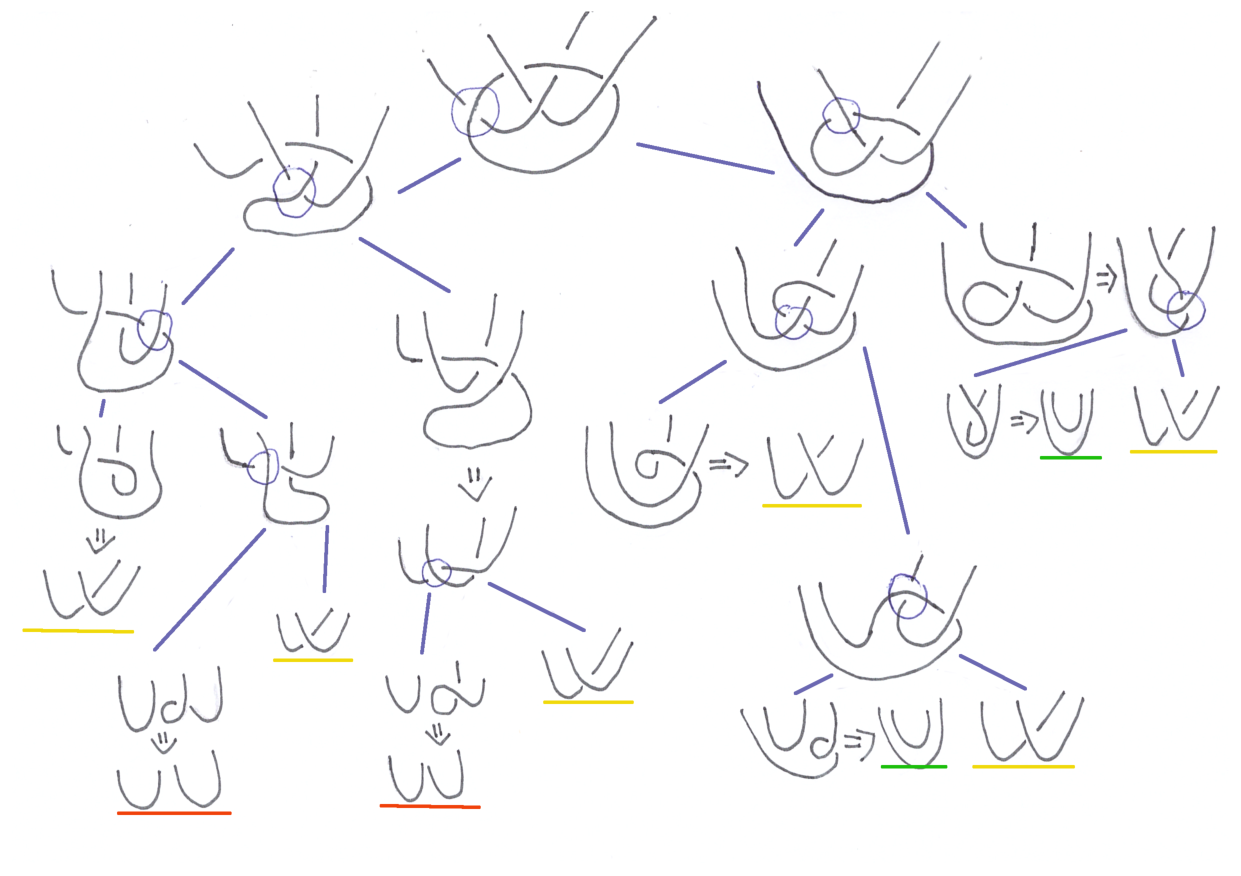
\includegraphics[scale=0.68]{../img/horniodhad}
\caption{Průběh} \label{prubehhorni}
\end{figure}

Na obrázku~\ref{prubehhorni} je znázorněn strom s průběhem algoritmu na diagramu $B_k$ takový, že jsou postupně odstraňovány krajní kružnice. V kořeni se nachází úsek diagramu obsahující nějakou krajní kružnici. Zakroužkováním je označeno křížení, které bylo vybráno k rozpojení (volba křížení odpovídá variantám A i B a samozřejmě i RND). Šipkou je znázorněno, pokud dojde k rozmotání diagramu. Žlutě podtržení potomci jsou diagramy $B_{k-1}$. Červeně a zeleně podržení potomci jsou synové diagramu $B_{k-1}$, jak je vidět na obrázku~\ref{rozdvojeni}.

\begin{figure}[p] \centering
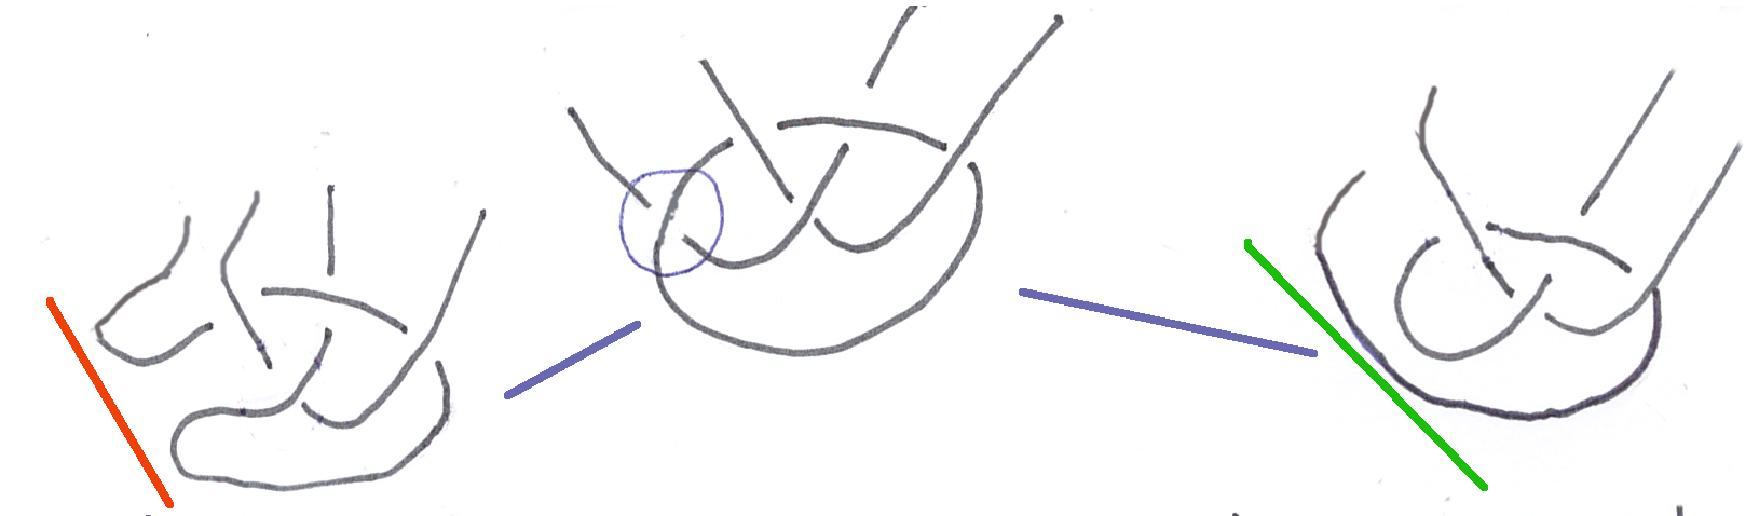
\includegraphics[scale=0.7]{../img/rozdvojeni}
\caption{Rozdvojení}  \label{rozdvojeni}
\end{figure}

Dohromady tedy z diagramu $B_k$ rozpojováním vznikne šest diagramů $B_{k-1}$ a čtyři synové $B_{k-1}$. Výpočet závorkového polynomu diagramu $B_k$ je tedy těžký alespoň jako výpočet polynomu osmi diagramů $B_{k-1}$. 

Časová složitost algoritmu na diagramu s $n$ kříženími splňuje rekurenci
$$ T(n) = 8T(n-4) + C_1 n + C_0  $$
pro jisté konstanty $C_0$, $C_1$.

Z toho plyne, že $T(n) = \Omega(8^{\frac{n}{4}})  =  \Omega(2^{0.75 n})$. \\

Na výpočet Jonesova polynomu ze závorkového polynomu je potřeba pouze lineární počet operací, tedy i výpočet Jonesova polynomu má časovou složitost $\Omega(2^{0.75n})$.
\end{dukaz}

%%% Třetí kapitola

\chapter{Třetí}

\section{Co v ní}
Experiment, náhodné uzly, experimenty na jinych uzlech, různé algoritmy?
Zatim urcite nechat probehnout na dvanacti uzlech,
Pak na velkych nahodnych uzlech
Pak na nejakych specialnich uzlech podle meho uvazeni
Jak generuji nahodne uzly
Bylo by zajímavé identifikovat, pro které typy uzlů je algoritmus efektivní a pro které naopak dosahuje nejhorších výsledků.

\chapter*{Závěr}
\addcontentsline{toc}{chapter}{Závěr}

Nezapomenout dělat závěry průběžně. Shrnovat to. Já vím, co to znamená, ale oni ne! Takže do toho.

Takže hlavně shrnovat ty složitosti. Že to na některých uzlech běží dobře. Nachám to běžet na torus.

Myslet meta - co mi tak ještě chybí, aby to dobře shrnulo Jonesův polynom?
Jakože je to práce o něm? Nebo mám jenom studovat?

Nedělitelné mezery

Labelování definic, obrázků, vět...

%%% Seznam použité literatury
%%% Seznam použité literatury (bibliografie)
%%%
%%% Pro vytváření bibliografie používáme bibTeX. Ten zpracovává
%%% citace v textu (např. makro \cite{...}) a vyhledává k nim literaturu
%%% v souboru literatura.bib.
%%%
%%% Příkaz \bibliographystyle určuje, jakým stylem budou citovány odkazy
%%% v textu. V závorce je název zvoleného souboru .bst. Styly plainnat
%%% a unsrt jsou standardní součástí latexových distribucí. Styl czplainnat
%%% je dodáván s touto šablonou a bibTeX ho hledá v aktuálním adresáři.

% \bibliographystyle{czplainnat}    %% Autor (rok) s českými spojkami
% \bibliographystyle{plainnat}    %% Autor (rok) s anglickými spojkami
\bibliographystyle{unsrt}       %% [číslo]
%\bibliographystyle{czunsrt}  

\renewcommand{\bibname}{Seznam použité literatury}

%%% Vytvoření seznamu literatury. Pozor, pokud jste necitovali ani jednu
%%% položku, seznam se automaticky vynechá.
\nocite{*}
\bibliography{literatura}

%%% Kdybyste chtěli bibliografii vytvářet ručně (bez bibTeXu), lze to udělat
%%% následovně. V takovém případě se řiďte normou ISO 690 a zvyklostmi v oboru.

% \begin{thebibliography}{99}
%
% \bibitem{lamport94}
%   {\sc Lamport,} Leslie.
%   \emph{\LaTeX: A Document Preparation System}.
%   2. vydání.
%   Massachusetts: Addison Wesley, 1994.
%   ISBN 0-201-52983-1.
% 
% \end{thebibliography}


%%% Obrázky v bakalářské práci
%%% (pokud jich je malé množství, obvykle není třeba seznam uvádět)
\listoffigures

%%% Tabulky v bakalářské práci (opět nemusí být nutné uvádět)
%%% U matematických prací může být lepší přemístit seznam tabulek na začátek práce.
\listoftables

%%% Použité zkratky v bakalářské práci (opět nemusí být nutné uvádět)
%%% U matematických prací může být lepší přemístit seznam zkratek na začátek práce.

%\chapwithtoc{Seznam použitých zkratek}

%ja
\listofalgorithms
\addcontentsline{toc}{chapter}{Seznam algoritmů}


%%% Přílohy k bakalářské práci, existují-li. Každá příloha musí být alespoň jednou
%%% odkazována z vlastního textu práce. Přílohy se číslují.
%%%
%%% Do tištěné verze se spíše hodí přílohy, které lze číst a prohlížet (dodatečné
%%% tabulky a grafy, různé textové doplňky, ukázky výstupů z počítačových programů,
%%% apod.). Do elektronické verze se hodí přílohy, které budou spíše používány
%%% v elektronické podobě než čteny (zdrojové kódy programů, datové soubory,
%%% interaktivní grafy apod.). Elektronické přílohy se nahrávají do SISu a lze
%%% je také do práce vložit na CD/DVD. Povolené formáty souborů specifikuje
%%% opatření rektora č. 72/2017.
%\appendix
%\chapter{Přílohy}

%\section{První příloha}

\openright
\end{document}
